%%%
%
% $Autor: Nayan $
% $Date: 2026-04-27 12:00:00Z $
% $File: ARIMA.tex $
% $Version: 1 $
%
% Project: Time Series CPI Forecasting
%
%%%

\chapter{AutoRegressive Integrated Moving Average (ARIMA)}
\label{ch:arima}

\section{Description}
The AutoRegressive Integrated Moving Average (ARIMA) model is one of the standard statistical tools for analyzing and forecasting univariate time series \cite{Box2015,Hyndman2021}. Its main idea is simple: future values are explained using past values, past forecast errors, and a differencing step that helps remove non-stationary trend behavior. In this report, ARIMA serves as the main non-seasonal baseline against which the more explicitly seasonal models are compared. Figure~\ref{fig:arima_tikz} illustrates the general modeling logic.

Let $y_t$ be the original series and $y'_t$ be the differenced series. A simplified ARIMA representation can be written as:
\begin{equation}
    y'_t = c + \phi_1 y'_{t-1} + \dots + \phi_p y'_{t-p} + \theta_1 \epsilon_{t-1} + \dots + \theta_q \epsilon_{t-q} + \epsilon_t
\end{equation}
The variables and coefficients in this formulation can be interpreted as follows:
\begin{itemize}
    \item \textbf{$y_t$ and $y'_t$:} the original observation at time $t$ and the differenced observation at time $t$.
    \item \textbf{$c$:} a constant drift or intercept term.
    \item \textbf{$\epsilon_t$:} the random error at time $t$, usually interpreted as white noise.
    \item \textbf{AutoRegressive (AR - $p$):} captures how strongly the current value depends on a selected number of past values.
    \item \textbf{Integrated (I - $d$):} applies differencing $d$ times to reduce trend and move the series closer to stationarity.
    \item \textbf{Moving Average (MA - $q$):} captures how current values depend on past forecast errors.
\end{itemize}

\begin{figure}[htbp]
\centering
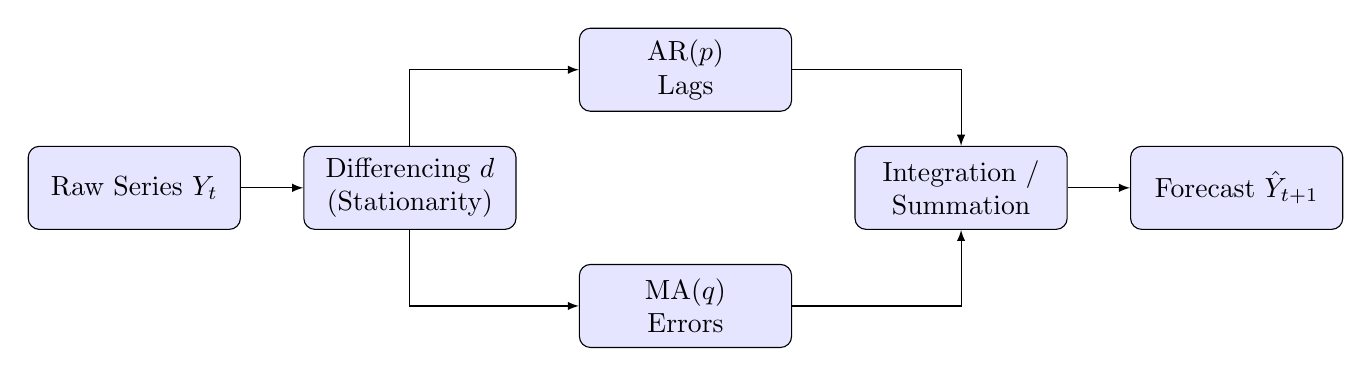
\begin{tikzpicture}[
    block/.style={rectangle, draw, fill=blue!10, text width=7em, text centered, rounded corners, minimum height=3em},
    line/.style={draw, -latex}
]
    \node [block] (input) at (0,0) {Raw Series $Y_t$};
    \node [block] (diff) at (3.5,0) {Differencing $d$ (Stationarity)};
    \node [block] (ar) at (7,1.5) {AR($p$) \\ Lags};
    \node [block] (ma) at (7,-1.5) {MA($q$) \\ Errors};
    \node [block] (sum) at (10.5,0) {Integration / Summation};
    \node [block] (output) at (14,0) {Forecast $\hat{Y}_{t+1}$};
    
    \draw [line] (input) -- (diff);
    \draw [line] (diff) |- (ar);
    \draw [line] (diff) |- (ma);
    \draw [line] (ar) -| (sum);
    \draw [line] (ma) -| (sum);
    \draw [line] (sum) -- (output);
\end{tikzpicture}

\caption{Architectural flowchart of an ARIMA($p,d,q$) model showing how the differenced signal is split into AutoRegressive and Moving Average paths before recombination. Source: own diagram based on the Box--Jenkins ARIMA formulation \cite{Box2015,Hamilton1994}.}
\label{fig:arima_tikz}
\end{figure}

\section{Applications}
ARIMA is widely used in settings where the main information comes from the history of a single variable. Typical examples include financial series, macroeconomic indicators, demand forecasting, epidemiological case counts, and short-term operational data. In economics especially, ARIMA is often used as a benchmark model because it is interpretable, well studied, and comparatively easy to estimate \cite{Box2015,Hamilton1994}.

\section{Relevance}
Within this project, ARIMA is important because it gives a clear baseline for forecasting Germany's Consumer Price Index. CPI data typically shows persistence, meaning that recent values still contain information about the next few months. ARIMA is well suited to capture that kind of autocorrelation. At the same time, it does not model seasonality as directly as SARIMA or ETS, which makes it a useful baseline: if a seasonal model performs better, that improvement can be interpreted more clearly.

\section{Hyperparameters}
The ARIMA model is defined by three primary hyperparameters, usually written as $(p, d, q)$:
\begin{itemize}
    \item \textbf{$p$ (lag order):} the number of past observations included in the autoregressive part. This is often informed by the Partial Autocorrelation Function (PACF), as shown in Figure~\ref{fig:arima_acf_pacf}.
    \item \textbf{$d$ (degree of differencing):} the number of times the raw series is differenced to move it closer to stationarity. This can be supported by tests such as the Augmented Dickey-Fuller (ADF) test.
    \item \textbf{$q$ (moving average order):} the number of lagged forecast errors included in the moving-average part. This is often informed by the Autocorrelation Function (ACF).
\end{itemize}

\begin{figure}[htbp]
    \centering
    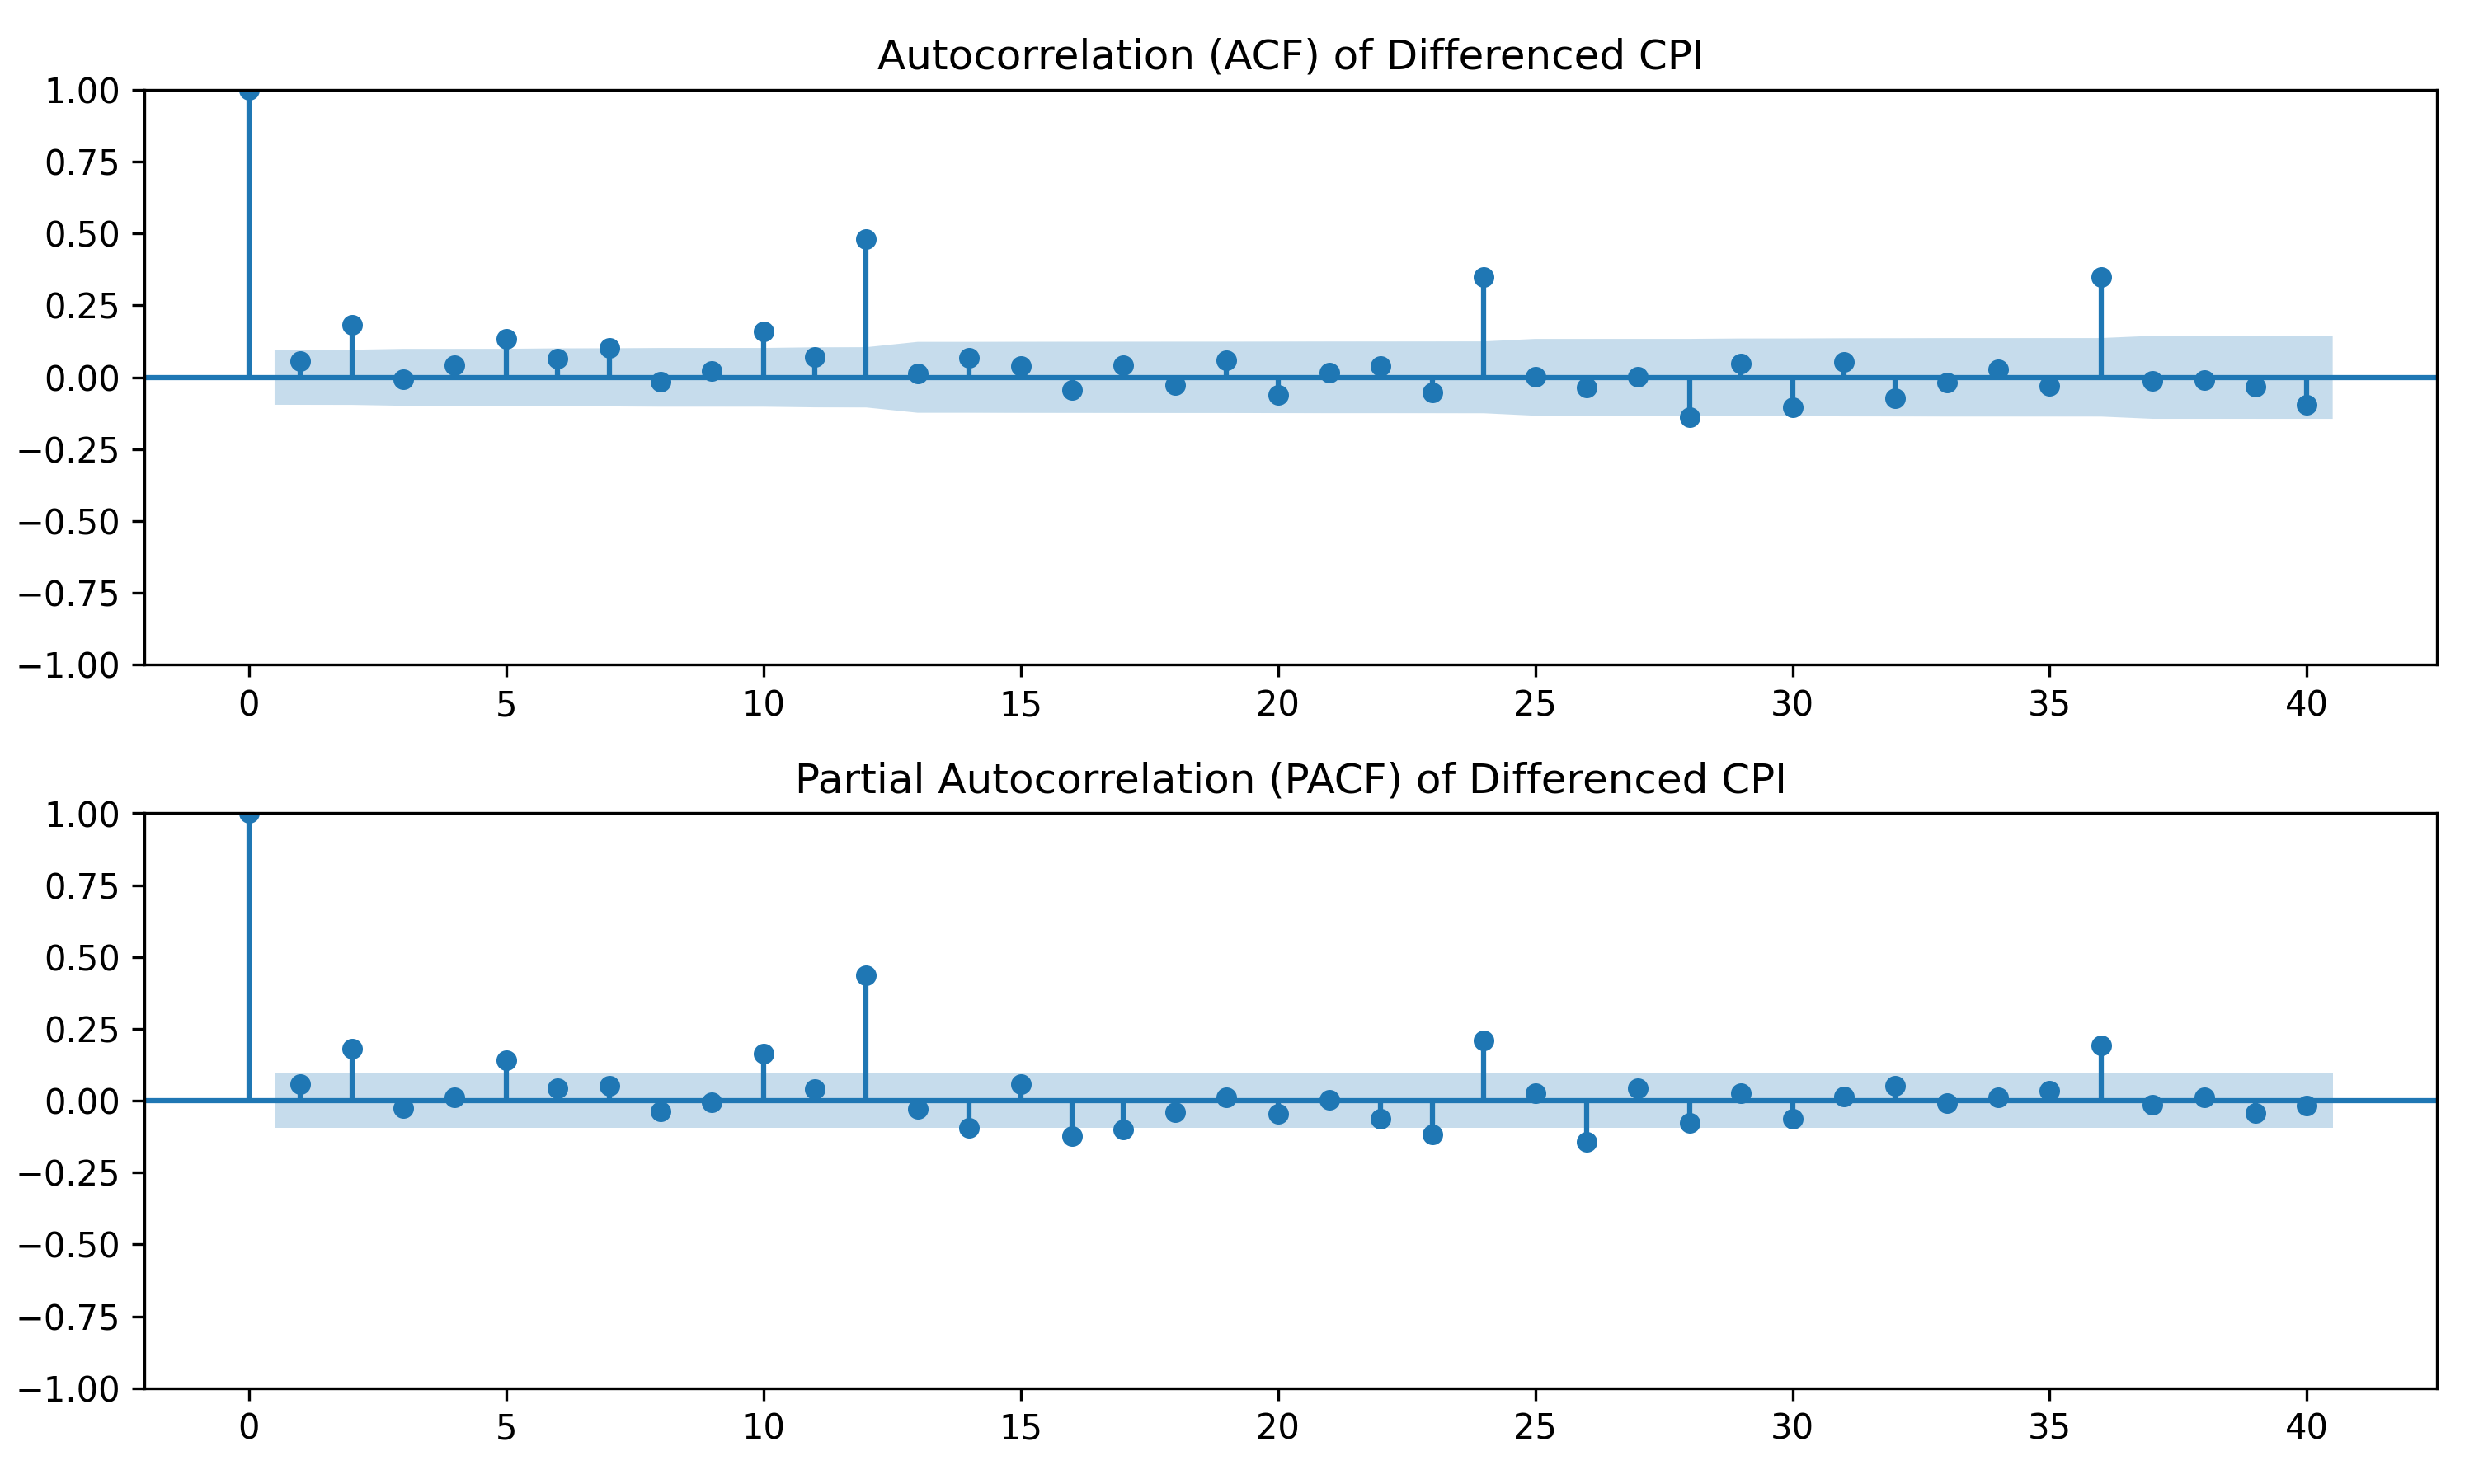
\includegraphics[width=0.9\textwidth]{../../Images/acf_pacf.png}
    \caption{Autocorrelation (ACF) and Partial Autocorrelation (PACF) plots used to empirically determine the Moving Average ($q$) and AutoRegressive ($p$) hyperparameters respectively. Source: own visualization based on Destatis GENESIS table 61111-0002 \cite{DestatisCPIQuality2023,DestatisCPIWeighting2023}.}
    \label{fig:arima_acf_pacf}
\end{figure}

\section{Requirements}
The most important practical requirement of ARIMA is that the input series should either be stationary or capable of being made approximately stationary through differencing \cite{Box2015,Hyndman2021}. In simple terms, this means that the underlying statistical behavior of the series should not drift too strongly over time once trend effects are removed. Figure~\ref{fig:arima_differencing} illustrates this idea by contrasting the upward-trending CPI series with its first-differenced version.

If the variance changes strongly over time, an additional transformation such as a logarithm or Box-Cox transform may also be useful before fitting the model. Standard ARIMA is not designed to model repeating seasonal structure directly, so series with clear seasonality are often better handled by SARIMA or by explicit deseasonalization.

\begin{figure}[htbp]
    \centering
    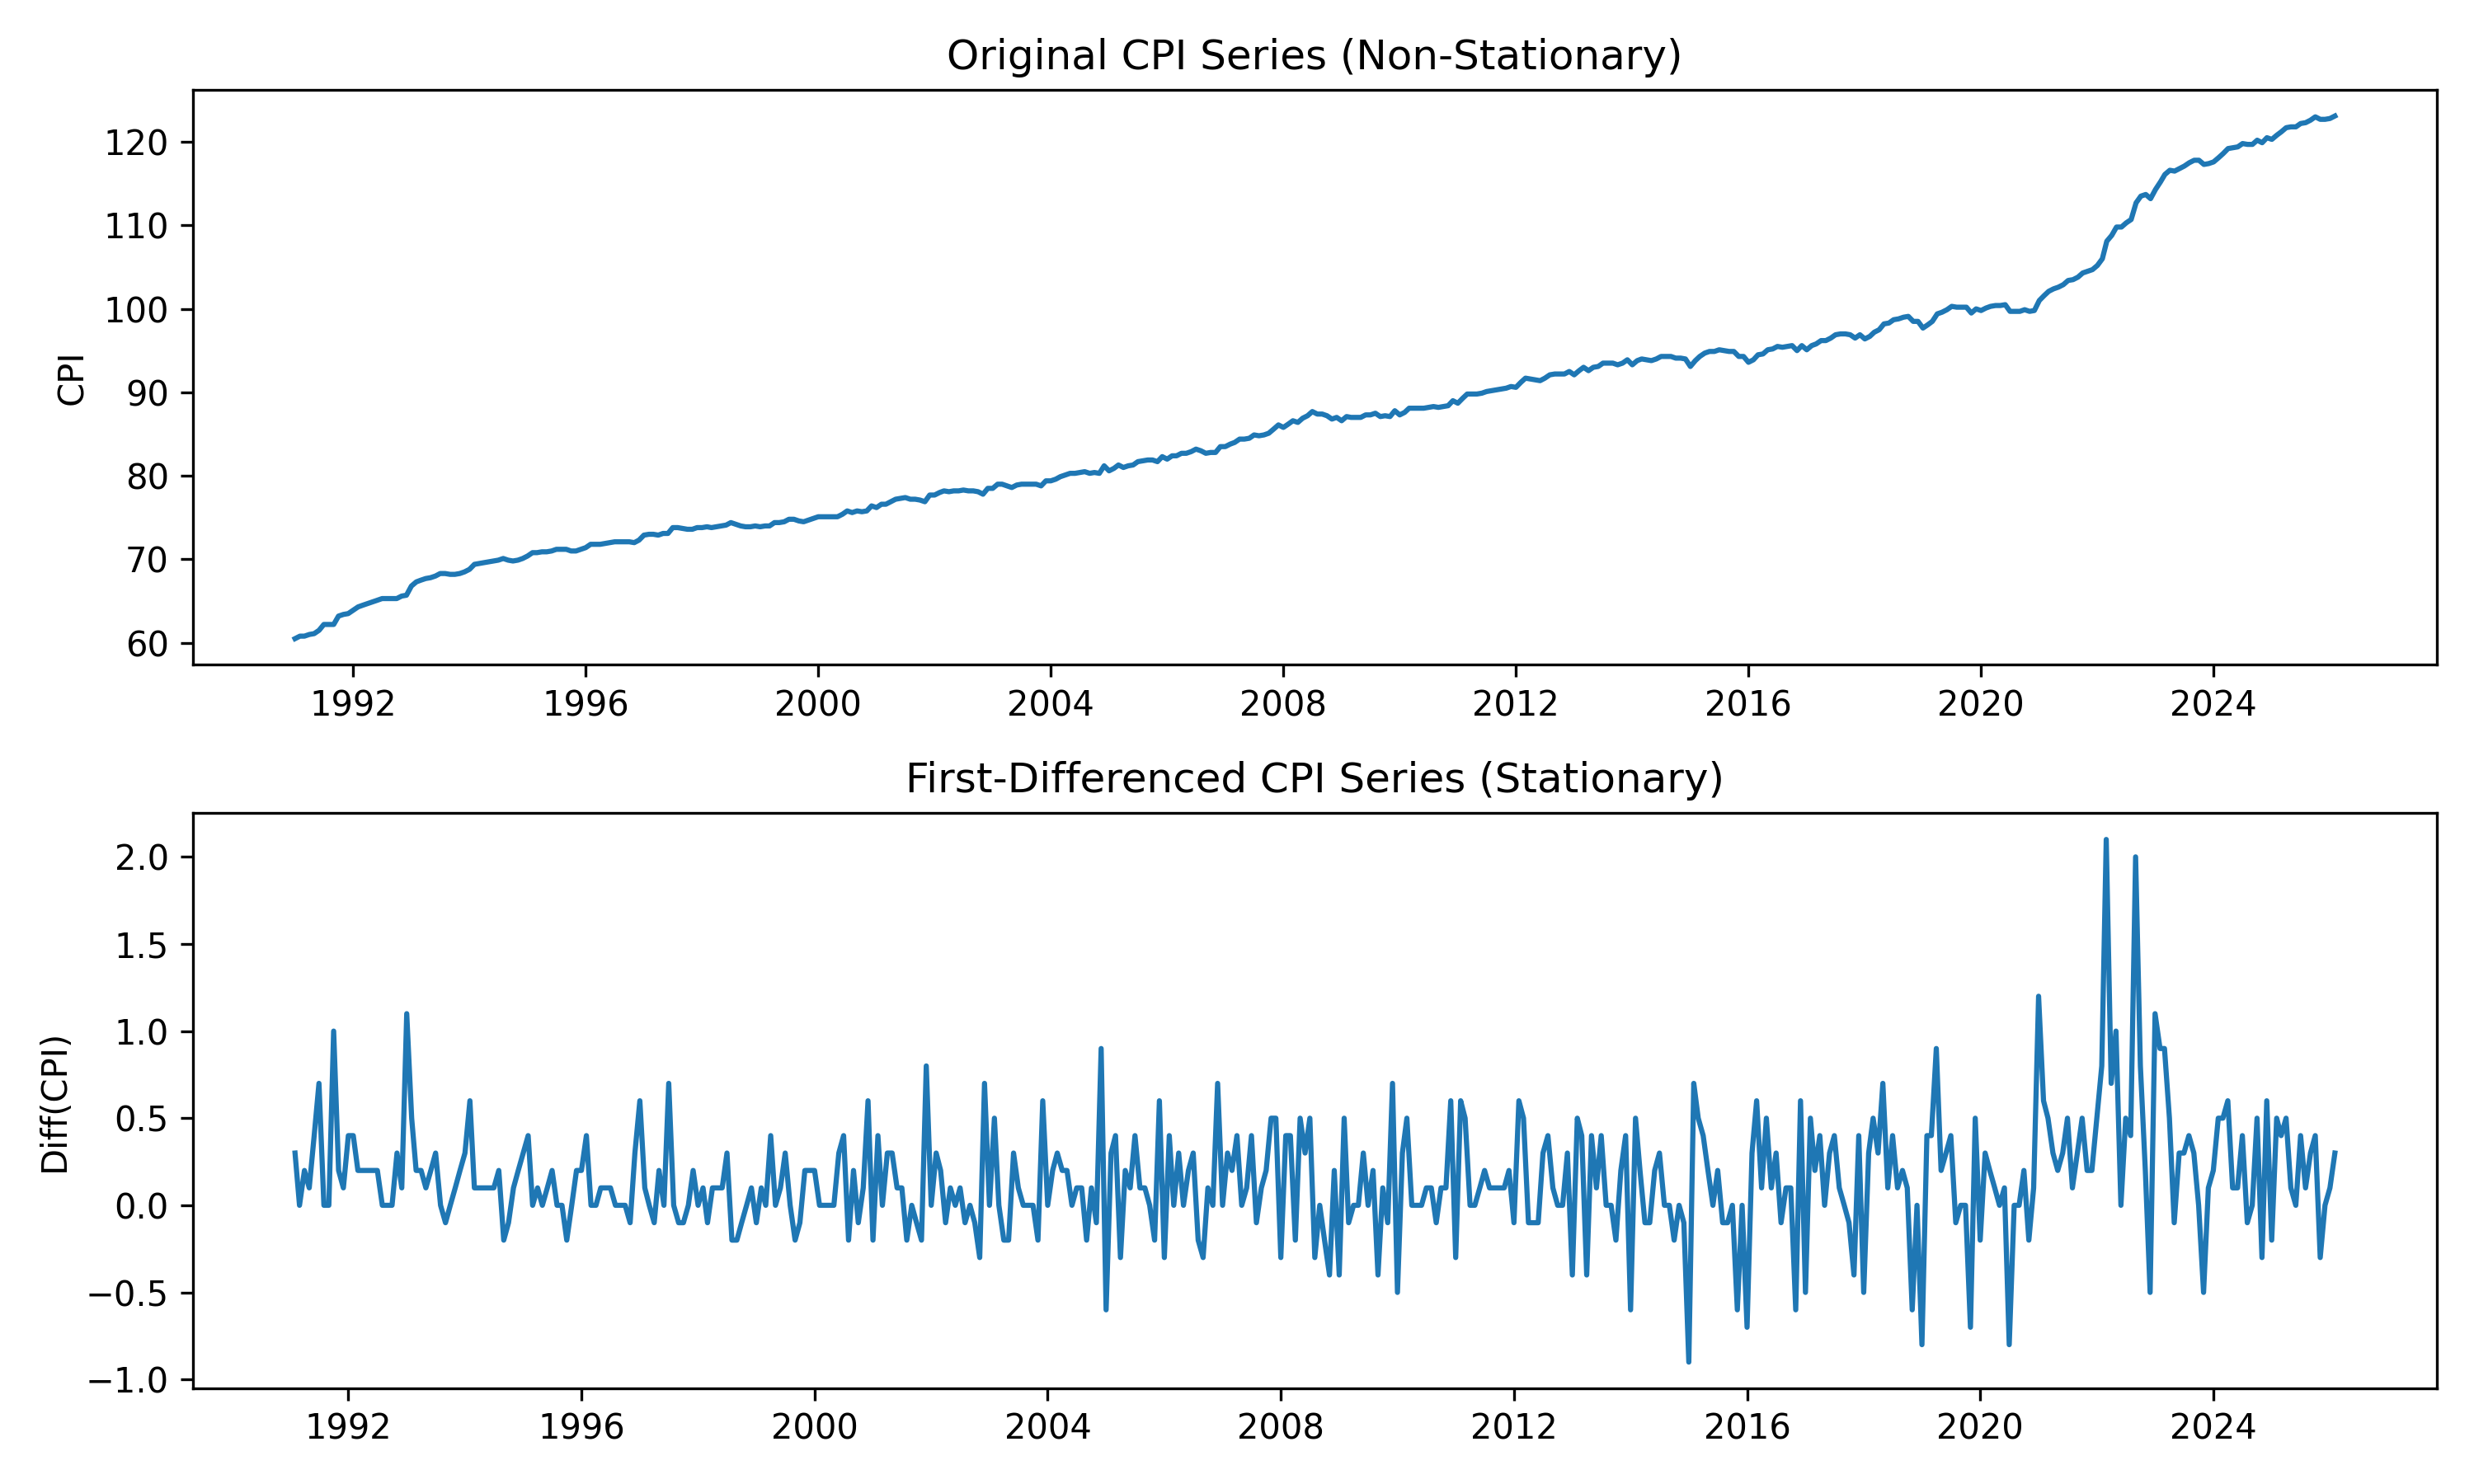
\includegraphics[width=0.9\textwidth]{../../Images/differencing.png}
    \caption{Original CPI Series (top) exhibiting a non-stationary upward trend, compared to the First-Differenced CPI Series (bottom) which achieves the stationarity required by ARIMA. Source: own visualization based on Destatis GENESIS table 61111-0002 \cite{DestatisCPIQuality2023,DestatisCPIWeighting2023}.}
    \label{fig:arima_differencing}
\end{figure}

\section{Input}
The model expects a univariate, equally spaced time series without missing values. In code, this is usually represented as a \texttt{pandas.Series} or \texttt{numpy.ndarray}, ordered chronologically and ideally indexed by a \texttt{DatetimeIndex} with a clear frequency such as monthly observations.

\section{Output}
The model outputs point forecasts for a specified number of future time steps. In addition, it provides estimated forecast uncertainty, which can be used to construct prediction intervals such as 95\% confidence bounds. This is helpful because a forecasting model should communicate not only its best estimate, but also how uncertain that estimate becomes as the forecast horizon grows.

\section{Example with a program}
The following Python snippet demonstrates the basic workflow for fitting and forecasting with an ARIMA model using \texttt{statsmodels}, assuming that stationarity checks have already been carried out:

\begin{Python}[caption={ARIMA Implementation using Statsmodels}, label={lst:arima_python}]
import pandas as pd
from statsmodels.tsa.arima.model import ARIMA

# Assume 'cpi_series' is a pandas Series with a monthly DatetimeIndex,
# and we have determined (p=1, d=1, q=1) via ACF/PACF and ADF tests.
cpi_series = pd.Series([105.1, 105.4, 105.8, 106.2, 106.5])

# Initialize the ARIMA model
model = ARIMA(cpi_series, order=(1, 1, 1))

# Fit the model using Maximum Likelihood Estimation (MLE)
fitted_model = model.fit()

# Forecast the next 12 periods (1 year)
forecast_result = fitted_model.get_forecast(steps=12)
predicted_means = forecast_result.predicted_mean
confidence_intervals = forecast_result.conf_int(alpha=0.05) # 95% CI

print("Forecasts:\n", predicted_means)
\end{Python}

\section{Further Reading}
\begin{itemize}
    \item Box, Jenkins, Reinsel, and Ljung, \textit{Time Series Analysis: Forecasting and Control} \cite{Box2015}
    \item Hyndman and Athanasopoulos, \textit{Forecasting: Principles and Practice} \cite{Hyndman2021}
\end{itemize}
